\chapter{Gráficas y Superficies}
La teoría de gráficas y el estudio de superficies son dos ramas de las matemáticas que, a primera vista, podrían parecer independientes. Sin embargo, a lo largo de este capítulo veremos que están profundamente relacionadas a través de la implementación de triangulaciones sobre superficies.

En particular, la representación de superficies mediante gráficas ofrece una nueva perspectiva que permite estudiar propiedades topológicas de los objetos que analizaremos en este trabajo. Una \textbf{gráfica} es un conjunto de \textbf{vértices} conectados mediante \textbf{aristas}, mientras que una \textbf{superficie} puede entenderse como un objeto que localmente es homeomorfo al plano \(\mathbb{R}^2\), como lo son la esfera o el toro. Al triangular una superficie —definición que abordaremos en este capítulo— es posible inducir una gráfica sobre ella. Esta construcción nos permite aplicar teoremas y algoritmos de la teoría de gráficas al estudio de superficies, facilitando, por ejemplo, su clasificación.

Este capítulo explora la relación entre ambas áreas, enfocándose en cómo la triangulación de superficies se convierte en una herramienta clave para comprender propiedades topológicas fundamentales, así como para implementar algoritmos relevantes en su análisis.

La primera parte, dedicada a definiciones y conceptos topológicos, se basa en los textos de \cite{munkres_topology_2000} y \cite{prieto_topologia_2003}. La segunda parte, enfocada en definiciones, conceptos y algoritmos relacionados con gráficas y su aplicación en superficies, toma como referencia los textos de \cite{haru}, \cite{diestel} y \cite{pressley}, los cuales serán también fundamentales en capítulos posteriores.

\section{Superficies}
Para comprender adecuadamente el objeto de estudio que se construye a lo largo de esta tesis, comenzaremos por introducir uno de los conceptos fundamentales que utilizaremos desde el inicio: el de superficie. Sin embargo, para poder definirlo con rigor, es necesario establecer previamente una serie de conceptos sobre los cuales se apoya esta definición.

El primer concepto clave es el de espacio topológico, que servirá como punto de partida y proporcionará el contexto necesario para este capítulo.

Algunas definiciones no se utilizarán en este capítulo ya que podrían considerarse básicas, pero para mantenerlas en contexto se incluyen en el apéndice \ref{ap:basicas}.

\begin{definition}(Espacio topológico)
    \\Sea $X$ un conjunto, una topología en $X$ es una familia $\mathcal{T}$ de subconjuntos abiertos de $X$, tal que cumple con los siguientes axiomas.
    \begin{enumerate}
        \item Si $\{T_i\}_{i \in \mathcal{I}} \subseteq \mathcal{T}$, $\mathcal{I}$ arbitrario, entonces \(\displaystyle \bigcup_{i \in \mathcal{I}} T_i \in \mathcal{T}\).
        \item Si $\{T_i\}_{i \in \mathcal{I}} \subseteq \mathcal{T}$, $\mathcal{I}$ finito, entonces $\displaystyle \bigcap_{i \in \mathcal{I}} T_i \in \mathcal{T}$
    \end{enumerate}
    Por ser $T$ la intersección de una familia vacía, entonces $X \in \mathcal{T}$, además por ser $\emptyset$ la unión de una familia vacía también yace en $\mathcal{T}$.
    \\ A la pareja $(X,\mathcal{T})$ se le denomina \textbf{\textit{espacio topológico}}.
\end{definition}

\begin{example}
    Sea $X$ un conjunto de dos elementos $X = \{x,y\}$, podemos definir una topología sobre este conjunto de la siguiente forma:
    \\Tomemos los conjuntos abiertos: $\mathcal{T} = \{X,\emptyset, \{x\} \}$
    \\Entonces observamos que:
    
    $\{x\} \cup X =X$, $\{x\} \cup \emptyset = \{x\}$,
    $X \cup \emptyset = X$, $\{x\} \cap X = \{x\}$,
    $\{x\} \cap \emptyset = \emptyset$, $X \cap \emptyset = \emptyset$
    
    Por tanto $(X,\mathcal{T})$ es un espacio topológico, en específico se le conoce como espacio topológico de Sierpiński.
    
\end{example}

\begin{definition}[Conjunto cerrado]
    Sea $X$ un espacio topológico. Decimos que un subconjunto $A$ de $X$ es \textbf{cerrado} si el conjunto $X-A$ es abierto.   
\end{definition}

\begin{example}
    Sea $A = \{x \times y | x\geq 0 \hspace{5pt} e \hspace{5pt} y \geq 0\} \subset \mathbb{R}^2$,entonces el conjunto A es cerrado.
    \begin{proof}
        Observamos que el complemento de $A$ es:
         \[\{x \times y \hspace{5pt}| x < 0 , y \geq 0\} \cup \{x \times y \hspace{5pt} | x \geq, y <0 \} \cup \{x \times y  \hspace{5pt}| x<0 , y <0 \}\] es decir \[\{x \times y \hspace{5pt}| x <0 , y \in \mathbb{R}\} \cup \{x \times y\hspace{5pt} | x \in \mathbb{R} \times y < 0\}\] lo cual es equivalente a  \[(- \infty , 0) \times \mathbb{R} \cup \mathbb{R} \times (0, \infty)\] , como cada uno de ellos es abierto y la unión de abiertos es abierta, entonces el complemento de $A$ es abierto y por lo tanto $A$ es un conjunto cerrado.
    \end{proof}

\end{example}

\begin{figure}[H]
    \centering
    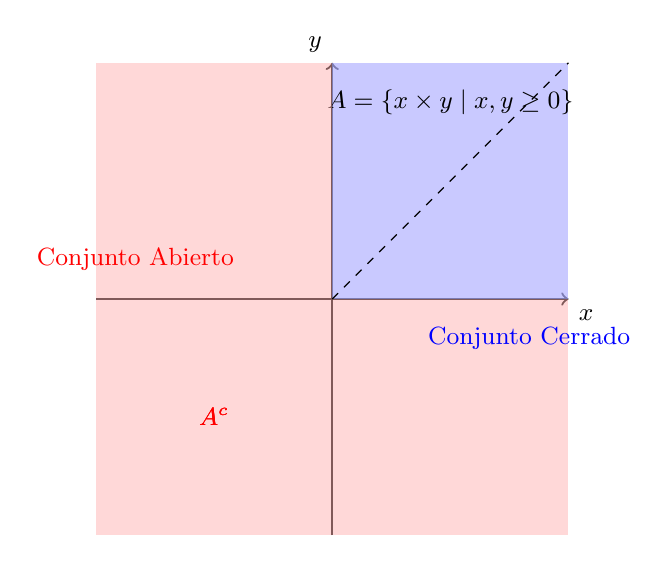
\begin{tikzpicture}
        % Ejes coordenados
        \draw[thick,->] (-3,0) -- (3,0) node[anchor=north west] {\small $x$};
        \draw[thick,->] (0,-3) -- (0,3) node[anchor=south east] {\small $y$};
    
        % Región del conjunto A (x*y con x,y >= 0)
        \fill[blue!30,opacity=0.7] (0,0) rectangle (3,3);
        \node at (1.5,2.5) {\small $A = \{x \times y \mid x, y \geq 0\}$};
    
        % Región del complemento A^c (parte negativa)
        \fill[red!30,opacity=0.5] (-3,-3) rectangle (0,0);
        \node[red] at (-1.5,-1.5) {\small $A^c$};
        \fill[red!30,opacity=0.5] (-3,3) rectangle (0,0);
        \node[red] at (-1.5,-1.5) {\small $A^c$};
        \fill[red!30,opacity=0.5] (3,-3) rectangle (0,0);
        \node[red] at (-1.5,-1.5) {\small $A^c$};
    
        % Etiquetas
        \node[blue] at (2.5,-0.5) {\small Conjunto Cerrado};
        \node[red] at (-2.5,0.5) {\small Conjunto Abierto};
    
        % Línea divisoria en x=0 e y=0
        \draw[dashed] (0,0) -- (3,3);
    \end{tikzpicture}
    \label{fig:cerrado}
    \caption{Ilustración del suconjunto $A$}
    
\end{figure}

\begin{definition}[Interior de un conjunto]
    Sea $X$ un espacio topológico y $A$ un subconjunto de $X$.
    El \textbf{interior} de $A$ se define como la unión de todos los conjuntos abiertos contenidos en $A$, es decir \[
    Int A = \displaystyle \bigcup_{i \in \mathcal{I}} A_i \hspace{5pt} | \hspace{5pt} A_i \subset A\] con $A_i$ abierto para $i \in \mathcal{I}$.   
\end{definition}

\begin{definition}[Cerradura de un conjunto]
    Sea $X$ un espacio topológico y $A$ un subconjunto de $X$.
    La \textbf{cerradura} de $A$ se define como la intersección de todos los conjuntos cerrados que conitienen a $A$, es decir \[
    \bar{A} = \displaystyle \bigcap_{i \in \mathcal{I}} A_i \hspace{5pt} | \hspace{5pt} A \subset A_i\] con $A_i$ cerrado para $i \in \mathcal{I}$.
\end{definition}

\begin{definition}[Frontera de un conjunto]
    Sea $X$ un espacio topológico y $A$ un subconjunto de $X$. Un punto $x \in \bar{A} \cap \overline{X-A} $ se denomina \textbf{punto frontera} de $A$; al conjunto  $\bar{A} \cap \overline{X-A}$ se le llama \textbf{frontera} de $A$.
    
\end{definition}

\begin{definition}(Espacio de Hausdorf)
    \\Sea $(X,\mathcal{A})$ un espacio topológico.Se dice que $X$  es un \textbf{Espacio de Hausdorf}, si para cada par $x_1, x_2$ de puntos distintos de $X$, existen vecindades $U_1,U_2$ de $x_1,x_2$ respectivamente, que son ajenas. Es decir $U_1 \cap U_2 = \emptyset$
\end{definition}

\begin{definition}(Cubierta abierta)
    \\Sea $X$ un espacio topológico, sea $\mathcal{A} = \{\mathcal{A}_i\}_{i \in \mathcal{I}}$ una familia de subconjuntos abiertos de $X$.
    \\Se dice que $\mathcal{A}$ es una \textbf{cubierta abierta} de $X$ si $X \subseteq \displaystyle \bigcup_{i \in \mathcal{I}} \{\mathcal{A}_i\} $
    
\end{definition}

\begin{definition}(Subcubierta finita)
    Sea $X$ un espacio topológico, sea $\mathcal{A}$ una cubierta abierta de $X$. 
    \\Decimos que $\mathcal{A}'$ es una subcubierta de $\mathcal{A}$ si $\mathcal{A}' \subset \mathcal{A}$, en particular si $\mathcal{A}'$ es finito, entonces es una \textbf{subcubierta finita}.
    
\end{definition}

\begin{definition}(Espacio Compacto)
    \\Sea $X$ un espacio topológico, se dice que $X$ es \textbf{compacto} si de cada cubierta abierta podemos extraer una subcubierta finita de $X$.
\end{definition}

\begin{example}
    Sea $X = \{0\} \cup \{ \frac{1}{n} \hspace{5pt} | \hspace{5pt} n \in \mathbb{Z}_{+} \}$ un subespacio de $\mathbb{R}$.
    \\Demostraremos a continuación que el espacio $X$ es un espacio compacto:
    \begin{proof}
        Sea $\{\mathcal{A}_{\alpha}\}$ una cubierta abierta de $X$, es decir $X \subseteq \displaystyle \bigcup_{\alpha} \mathcal{A}_{\alpha}$.
        \\Como $0 \in X$ y $\{\mathcal{A}_{\alpha}\}$ es cubierta abierta, entonces existe un entorno abierto $\mathcal{A}_0$ que contiene a 0, es decir , existe $\epsilon > 0$ tal que $(-\epsilon, \epsilon) \subseteq \mathcal{A}_0$.
        Notamos que, en particular existe un $N$ suficientemente grande tal que para todo $n>N$, se cumple que $\frac{1}{n} \in (-\epsilon,\epsilon)$, de ahí que los puntos de la forma $\frac{1}{N},\frac{1}{(N+1)},\frac{1}{(N+2)}, \dotsc $ están en $\mathcal{A}_0$, ahora los puntos restantes $1,2,\dotsc ,\frac{1}{N-1}$ notamos que son finitos y además están en algún $\mathcal{A}_{\alpha}$.Es decir están en una subcubierta finita.
        \\Por último notamos que la subcubierta finita de $X$ es de la forma $\mathcal{A}_0 \cup \mathcal{A}_{1} \cup \cdots \cup \mathcal{A}_{N-1}$ por tanto, $X$ es compacto.

    \end{proof}

\end{example}
\begin{figure}[H]
    \centering
    \begin{center}
        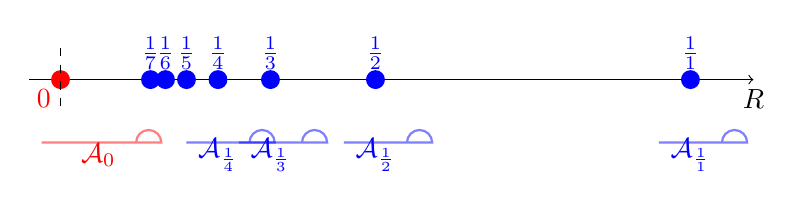
\begin{tikzpicture}[scale=8]
            \draw[->] (-0.05,0) -- (1.1,0) node[below] {$\mathbb{R}$};
            \filldraw[red] (0,0) circle (0.4pt) node[below left] {$0$};
    
            
            \foreach \n in {1,2,3,4,5,6,7} {
                \filldraw[blue] ({1/\n},0) circle (0.4pt) node[above] {$\frac{1}{\n}$};
            }
    
            % Indicador de la sucesión que converge a 0
            \draw[dashed] (0,0.05) -- (0,-0.05);
    
            % Entorno abierto alrededor de 0
            \draw[red,thick,opacity=0.5] (-0.03,-0.1) -- (0.12,-0.1) arc[start angle=180, end angle=0, radius=0.02] -- cycle;
            \node[red] at (0.06,-0.12) {$\mathcal{A}_0$};
    
            % Entornos abiertos para algunos puntos
            \foreach \n in {1,2,3,4} {
                \draw[blue,thick,opacity=0.5] ({1/\n - 0.05},-0.1) -- ({1/\n + 0.05},-0.1) arc[start angle=180, end angle=0, radius=0.02] -- cycle;
                \node[blue] at ({1/\n},-0.12) {$\mathcal{A}_{\frac{1}{\n}}$};
            }
        \end{tikzpicture}
    \end{center}
    \label{fig:compacto}
    \caption{Ilustración de la compacidad del espacio $X$}
    
    
\end{figure}

\begin{definition}(Base de vecindades)
    \\Sea $X$ un espacio topológico y $x \in X$. Decimos que una familia $\mathcal{B}_x$ de vecindades de $x$ es una \textbf{base de vecindades} de $x$ si para cualquier vecindad $U$ de $x$ existe una vecindad $V \in  \mathcal{B}_x$ tal que $V \subset U$
\end{definition}

\begin{definition}(Base numerable)
    Sea un espacio toplógico $X$. Se dice que $X$ tiene una base numerable en $x$ si existe una base de vecindades numerable.

\end{definition}


\begin{definition}(Primer axioma de numerabilidad)
    Sea $X$ un espacio topológico. Se dice que $X$ satisface el primer axioma de numerabilidad o que es 1-numerable, si cumple que, cada punto de $X$ tiene una base de vecindades numerable.
\end{definition}

\begin{definition}(Segundo axioma de numerabilidad)
    Sea $X$ un espacio topológico, se dice que $X$ satisface el segundo axioma de numerabilidad, o que es 2-numerable, si la topología $X$ admite una base numerable.
\end{definition}

\begin{example}
    Observamos que en la topología uniforme $\mathbb{R}^\omega$ satisface el primer axioma de numerabilidad por ser metrizable.Sin embargo no satisface el segundo. Para comprobar este hecho mostraremos que si $X$ es un espacio que tiene base numerable $\mathcal{B}$, entonces cualquies subespacio discreto $A$ de $X$ debe ser numerable. Elijamos para cada $a \in A$ un elemento $B_a$ de la base que interseque a $A$ unicamente en el punto a, si a y b son distintos de A , los conjuntos $B_a$ y $B_b$ son distintos , puesto que el primero contiene a $a$ y el segundo no. Se sigue que l aplicación $a \rightarrow B_a$ es una inyección de $A$ en $\mathcal{B}$, por lo que $A$ debe ser numerable.
    Ahora bien, el subespacio $A$ de $\mathbb{R}^\omega$ formado por todas las suscesiones de ceros y unos no es umerable y tiene la topologóa discreta porque $\bar{\rho}(a,b) = 1$ no tiene una base numerable.
\end{example}


\begin{definition}(Variedad topológica)
    Un espacio topológico $X$, de Hausdorff, 2-numerable es una \textbf{variedad topológica} de dimensión n, también llamada n-variedad, si cada punto $x \in X$ tiene una vecindad homeomorfa a un abierto $U$ en la n-bola cerrada $\mathbb{B}^n$
\end{definition}

\begin{definition}
    (Superficie)\\
        Una $2-variedad$ $S$ es una superficie. Si es compacta y no tiene frontera se le llama \textbf{Superfice cerrada}
\end{definition}

\begin{example}

Sea $\mathrm{S}$ = $\{(x,y,z) \in \mathbb{R}^3 | z = x^2 - y^2 \}$
Demostraremos que $\mathrm{S}$ es una superficie, entonces , tenemos que demostrar que para cada punto $p \in \mathrm{S}$ existen conjuntos, $U \in \mathbb{R}^2$, $W \in \mathbb{R}^3$ abiertos tal que $p \in W \cap S$ y que existe $h: S\cap W \subset \mathbb{R}^3 \rightarrow U \subset \mathbb{R}^2$ tal que $h$ es un homeomorfismo.

\begin{proof}
    Sea $p = (x_0,y_o,z_0) \in S$ entonces por definición $ z_0 = x_0^2 - y_0^2$, por otro lado definimos a $W \subset \mathbb{R}^3$ como la bola abierta centrada en $p$ de radio $r$ $\mathcal{B}_p(r)$ y a $U \subset \mathbb{R}^2$ como la vecindad alrededor de $(x_0,y_0)$, $V(x_0,y_0)$.\\
    Definamos ahora la función $\Pi: \mathrm{S}\cap W \rightarrow U$ dada por:

    \[
    \Pi(x,y,x) = (x,y)
    \]
    Es decir la función proyección restringida a $\mathrm{S}\cap W$, ahora notemos lo siguiente:

    \begin{itemize}
        \item $\Pi$ es una función continua ya que es la restricción de la función proyección que es continua en $\mathbb{R}^3$.
        \item $\Pi$ es inyectiva pues, dado $u=(x_1,y_1,z_1),w=(x_2,y_2,z_2) \in S\cap W$ tenemos que :
        \begin{align*}
        \Pi(x_1,y_1,z_1) &= \Pi(x_2,y_2,z_2) \Rightarrow \\
        (x_1,y_1) &= (x_2,y_2) \Rightarrow \\
        x_1 = x_2 &, y_1 = y_2
        \end{align*}
        Por otro lado como $u,w \in S$ entonces:
        \begin{align*}
            z_1 = x_1^2 - y_1^2 = x_2^2 - y_2^2 = z_2
        \end{align*}
        Es decir :
        \begin{align*}
            u = (x_1,y_1,z_1) = (x_2,y_2,z_2) = w
        \end{align*}
        Por tanto $\Pi$ es inyectiva.
        \item Sea $(x,y) \in U$ entonces notamos que existe un punto en $p \in S \cap W$ dado por $p = (x,y,x^2-y^2)$ por tanto $\Pi$ es sobreyectiva.
        \item Notamos que $\Pi^{-1}$ está dada por $\pi^{-1}(x,y) = (x,y,x^2-y^2)$, como las componentes $x,y$ son continuas y $x^2 - y^2$ es una combinación lineal de componentes continuas entonces $\Pi ^{-1}(x,y)=(x,y,x^2 - y^2)$ es continua
    \end{itemize}
    Por tanto $\Pi$ es un homeomorfismo y por tanto $S \cap W$ es homeomorfo a $U$ y por lo tanto $S$ es una superficie.
\end{proof}


\begin{figure}[H]
	\centering
    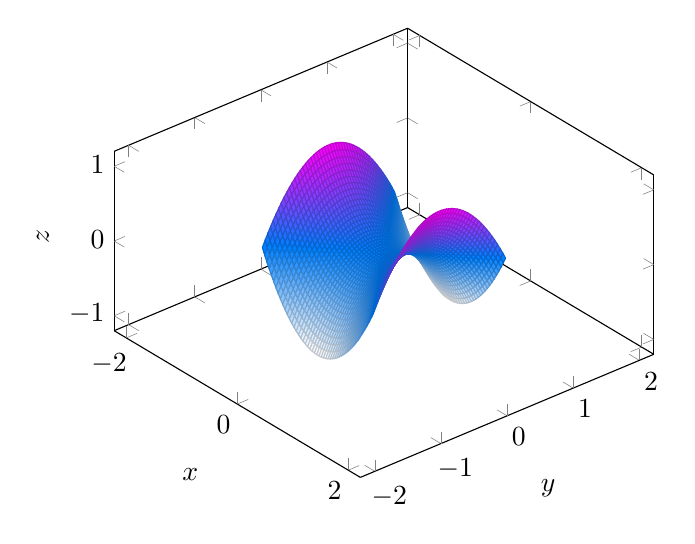
\begin{tikzpicture}
    \begin{axis}[
        view={50}{30}, % Ángulo de visión
        axis equal,
        colormap/cool,
        xlabel={$x$},
        ylabel={$y$},
        zlabel={$z$},
    ]
    \addplot3[surf, samples=50, domain=-1:1, y domain=-1:1] 
        {x^2 - y^2}; % Ecuación de la silla de montar
    \end{axis}

\end{tikzpicture}
    \label{fig:silla}
    \caption{Ejemplo de superficie en $\mathbb{R}^3$ comúnmente conocida como "Silla de Montar"}
\end{figure}


\end{example}
Habiendo establecido una forma rigurosa de definir superficies, es útil explorar cómo podemos representar estas superficies mediante estructuras más manejables y adecuadas para los objetivos de esta tesis. Una técnica clave es la triangulación, que nos permite descomponer una superficie en elementos simples, como triángulos, preservando su estructura topológica. En este contexto, el teorema de triangulación de Radó desempeña un papel central, ya que garantiza que cualquier superficie puede ser triangulada. Este proceso nos permite asociar una gráfica a la superficie al considerar los vértices y aristas de la triangulación, facilitando su estudio como gráfica.

\begin{definition}(Triángulo curvo)\\
    Sea $X$ un espacio de Hausdorff compacto. Un \textbf{triángulo curvo} en $X$ es un par $(A,h)$ formado por un subespacio $A$ de $X$ y un homeomorfismo $h: T \rightarrow A$ donde $T$ es una región triangular cerrada del plano. 
    Si $e$ es una arista de $T$, entonces $h(e)$ es una artista de $A$: si $v$ es in vértice de $T$,entonces $h(v)$ es un vértice de $A$.
    
\end{definition}


\begin{figure}[H]
	\centering
    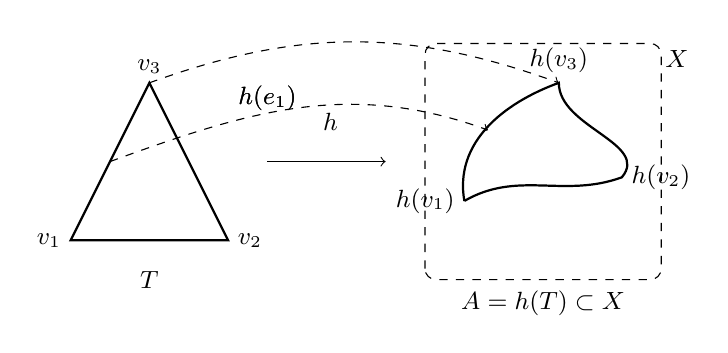
\begin{tikzpicture}

        % Triángulo en el plano
        \coordinate (A) at (0,0);
        \coordinate (B) at (2,0);
        \coordinate (C) at (1,2);

        \draw[thick] (A) -- (B) -- (C) -- cycle;
        \node[left] at (A) {\small $v_1$};
        \node[right] at (B) {\small $v_2$};
        \node[above] at (C) {\small $v_3$};

        \node at (1,-0.5) {\small $T$};

        % Flecha que indica el homeomorfismo
        \draw[->] (2.5,1) to[out=0,in=180] (4,1);
        \node at (3.3,1.5) {\small $h$};

        % Imagen del triángulo curvo en X
        \coordinate (A2) at (5,0.5);
        \coordinate (B2) at (7,0.8);
        \coordinate (C2) at (6.2,2);

        \draw[thick] (A2) to[out=30,in=200] (B2) 
                     to[out=50,in=270] (C2) 
                     to[out=200,in=100] (A2);

        \node[left] at (A2) {\small $h(v_1)$};
        \node[right] at (B2) {\small $h(v_2)$};
        \node[above] at (C2) {\small $h(v_3)$};

        \node at (6,-0.8) {\small $A=h(T) \subset X$};

        % Correspondencias entre aristas
        \draw[dashed,->] (0.5,1) to[out=20,in=160] (5.3,1.4);
        \node at (2.5,1.8) {\small $h(e_1)$};

        \draw[dashed,->] (1,2) to[out=20,in=160] (6.2,2);
        \node at (2.5,1.8) {\small $h(e_1)$};

       

        % Espacio X
        \draw[rounded corners, dashed] (4.5,-0.5) rectangle (7.5,2.5);
        \node at (7.7,2.3) {\small $X$};

    \end{tikzpicture}
    \label{fig:Triangulo}
    \caption{Ejemplo de triángulo curvo}
\end{figure}

\begin{definition}(Triangulación)\\
    Sea $X$ un espacio topológico.Una \textbf{triangulación} de una superficie $X$ es una colección de triángulos curvos $A_1, \cdots , A_n$ en $X$ cuya unión es $X$, tal que para $i \neq j$, la intersección $A_i \cup A_j$ es: vacía, un vértice de ambos o una arista de ambos.  Si $X$ poseé una triangulación, se dira que $X$ es \textbf{triangulable}.
\end{definition}

\begin{figure}[H]
    \centering
    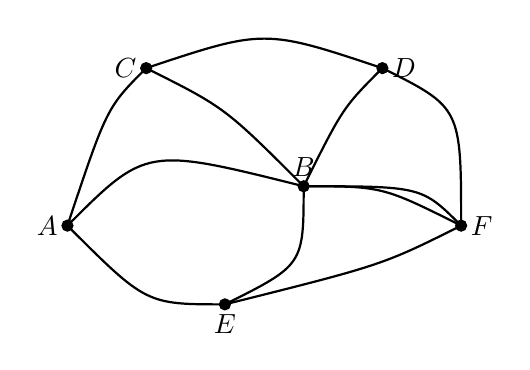
\begin{tikzpicture}
        % Definir los nodos de los vértices
        \coordinate (A) at (0,0);
        \coordinate (B) at (3,0.5);
        \coordinate (C) at (1,2);
        \coordinate (D) at (4,2);
        \coordinate (E) at (2,-1);
        \coordinate (F) at (5,0);
    
        % Dibujar los triángulos curvos
        \draw[thick] (A) .. controls (1,1) .. (B) .. controls (2,1.5) .. (C) .. controls (0.5,1.5) .. (A);
        \draw[thick] (B) .. controls (3.5,1.5) .. (D) .. controls (2.5,2.5) .. (C);
        \draw[thick] (B) .. controls (3,-0.5) .. (E) .. controls (1,-1) .. (A);
        \draw[thick] (B) .. controls (4,0.5) .. (F) .. controls (4,-0.5) .. (E);
        \draw[thick] (D) .. controls (5,1.5) .. (F) .. controls (4.5,0.5) .. (B);
        
        % Marcar los puntos
        \filldraw[black] (A) circle (2pt) node[left] {$A$};
        \filldraw[black] (B) circle (2pt) node[above] {$B$};
        \filldraw[black] (C) circle (2pt) node[left] {$C$};
        \filldraw[black] (D) circle (2pt) node[right] {$D$};
        \filldraw[black] (E) circle (2pt) node[below] {$E$};
        \filldraw[black] (F) circle (2pt) node[right] {$F$};
    
    \end{tikzpicture}
    \label{fig:Triangulación}
    \caption{Ejemplo de triangulación en una superficie}
\end{figure}

\begin{teorema}(Teorema de Radó)\\
    Toda superficie cerrada \textbf{S} es homeomorfa a ua superficie triangulada.
\end{teorema}

\section{Gráficas}
\begin{definition}[Gráfica] 
Una gráfica simple $G$ está definida por un par ordenado $G = (V,E)$, donde V es un conjunto cuyos elementos son llamados vértices (o nodos) de la gráfica y E un conjunto cuyos elementos son las aristas de la gráfica. Regularmente denotamos a $V$ y $E$ como $V(G)$ y $E(G)$ que hacen referencia a la gráfica G, entonces $G=(V(G),E(G))$
Definimos a $E$ como:
\begin{center}
$E(V)$ = $\{\{u,v\} | u,v \in V, u \neq v \}$
\end{center}
Usualmente denotamos al par $\{u,v\}$ simplemente como $uv$.
\end{definition}

\begin{definition}[Orden y tamaño] 
Para una gráfica $G$ , tenemos que:
\begin{enumerate}
    \item $\nu_{G}$ = $|\mathbf{V(G)}|$ es llamado el orden de $G$.
    \item $\varepsilon_{G}$ = $|\mathbf{E(G)}|$ es llamado  el tamaño de $G$.
    \item Para cada arista $e = uv \in E$ los vértices $u$ y $v$ son llamados extremos de la arista.
    \item Los vértices $u$ y $v$ son adyacentes o vecinos si $e = uv \in E$.
    \item Dos aristas $e_1 = uv$ y $e_2 = uw$ tienen un extremo común, entonces son adaycentes entre sí.
\end{enumerate}
\end{definition}

\begin{center}
\begin{figure}[H]
    \centering
    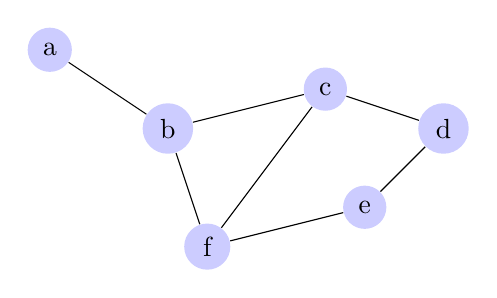
\begin{tikzpicture}
  [scale=.5,auto=left,every node/.style={circle,fill=blue!20}]
  \node (n6) at (1,10) {a};
  \node (n4) at (4,8)  {b};
  \node (n5) at (8,9)  {c};
  \node (n1) at (11,8) {d};
  \node (n2) at (9,6)  {e};
  \node (n3) at (5,5)  {f};

  \foreach \from/\to in {n6/n4,n4/n5,n5/n1,n1/n2,n3/n5,n2/n3,n3/n4}
    \draw (\from) -- (\to);

\end{tikzpicture}
    \caption{Ejemplo de gráfica simple G}
    \label{fig:G}
\end{figure}
\end{center}

\begin{flushleft}

En la figura \ref{fig:G} podemos observar que $\nu_{G}$ = 6, $\varepsilon_{G}$ =7, los extremos de la arista $ab$ son los vértices $a$ y $b$, también los vértices $a$ y $b$ son vecinos y por último las aristas $ab$ y $bf$ son adyacentes ya que comparten el vértice $b$.
\end{flushleft}


 

\subsection{Matriz de adyacencia}
\noindent Sabemos que las figuras planas mostradas en la sección anterior, son fácilmente comprensibles para nuestros ojos, pero al momento de crear algoritmos o de computarlas es muy costoso en términos de memoria por lo cual, es necesario el manejo de estos objetos de una forma un poco más \"comprensible\" para cualquier computadora, de esta forma nace la  \textbf{matriz de adyacencia} que definiremos a continuación.
\begin{definition}[Matriz de Adyacencia]
    Sea $V_G = \{v_1,...,v_n\}$ ordenado. 
    La matriz de adyacencia $\mathbf{A}$ de $\mathbf{G}$ está definida cómo \begin{center}
        $\mathbf{A}(\mathbf{G})$ = $\left[a_{ij}\right]$
    \end{center}
    donde:
    \begin{center}
        $a_{ij}$=$\left\lbrace\begin{array}{c} 1~si~v_iv_j \in \mathbf{E_G} \\0~si~no \end{array}\right.$
    \end{center}
\end{definition}
La matriz de adyacencia de la figura \ref{fig:G} quedaría de la siguiente forma:
\begin{center}
\begin{equation}
A(G) =
\begin{pmatrix}
0 & 1 & 0 & 0 & 0 & 0\\
1 & 0 & 1 & 0 & 0 & 1\\
0 & 1 & 0 & 1 & 0 & 1\\
0 & 0 & 1 & 0 & 1 & 0\\
0 & 0 & 0 & 1 & 0 & 1\\
0 & 1 & 1 & 0 & 1 & 0
\end{pmatrix}
\end{equation}
    
\end{center}

\subsection{Grado de un vértice}
\begin{definition}[Vecindario]
    Sea $v \in \mathbf{G}$ un vértice de la gráfica $\mathbf{G}$. El \textbf{vecindario} de $v$ es el conjunto dado por:
    \begin{center}
        $N_G(v)$ = $\{u \in G \hspace{5pt} | \hspace{5pt} vu \in \mathbf{E(G)}\}$
    \end{center}
    \end{definition}
    
    \begin{definition}[Grado de un vértice]
    El \textbf{grado} de $v$ es el numero de sus vecinos.
    \begin{center}
        $d_{G}(v)$ = $|N_G(v)|$.
    \end{center}  
    \end{definition}
    \noindent De la definición anterior podemos notar que para cualquier vértice $v$, podría suceder que $v$ no tenga vecinos o por el otro lado que el resto de los vértices de $G$ sean sus vecinos, recordando que $v$ no puede ser vecino de sí mismo. Así, se tiene que 
    \begin{center}
        0 $\leq$ $d_G(v)$ $\leq$ $n-1$
    \end{center} 
    donde $n$ es el orden la gráfica $G$.

    \begin{definition}[Vértice aislado]
    Cuando $d_G(v)$= 0 decimos que $v$ es un vértice aislado.
    \end{definition}
    
    \noindent Dada una gráfica $G = (V,E)$ con $V(G) = \{v_1,...,v_n\}$ sabemos que el conjunto:
    \[\{d_G(v_1),.\hspace{1pt} . \hspace{1pt}.\hspace{1pt},d_G(v_n)\}\]
    Es un conjunto finito de números naturales pues el conjunto V(G) lo es, entonces de esta forma podemos definir a $\delta(G)$ como el grado mínimo de G y $\Delta(G)$ como el grado máximo de G.

    \begin{definition}[Grado mínimo y grado máximo]
    Sea $G = (V,E)$ una gráfica simple, tenemos que;
    \begin{enumerate}
        \item  $\delta(G)$ = $min\{d_G(v_1),.\hspace{1pt}.\hspace{1pt}.\hspace{1pt},d_G(v_n)\}$ es el grado mínimo de $G$.
        \item $\Delta(G)$ = $max\{d_G(v_1),.\hspace{1pt}.\hspace{1pt}.\hspace{1pt},d_G(v_n)\}$ es el grado máximo de $G$.
    \end{enumerate}      
    \end{definition}

    \noindent Para la gráfica de la figura \ref{fig:G} tenemos que $\delta(G)$ = 1 y que $\Delta(G)$ = 3.


\begin{lemma}
    \textbf{(Lema del saludo de manos)}
    Para cada gráfica $G$ tenemos que:
 
        \[
\sum_{v \in V(G)}d_G (v) = 2 \hspace{5pt}\varepsilon_G
\]
Además, el número de vértices de grado impar es par.
   
\end{lemma}
\begin{proof}

\end{proof}

\begin{definition}[Grado promedio]
    Dada una gráfica $G$, definimos el \textbf{grado promedio} de G como:
    
         \[d(G) = \frac{1}{\nu_G}\sum_{v\in V(G)}d_G (v)\]
\end{definition}

    
    De ahí se reduce inmediatamente por \textbf{lema 5} que 
    
         \[d(G) = 2\hspace{3pt}\frac{\varepsilon_G}{\nu_G} \]



\begin{proposition}
Dada una gráfica $G$, tenemos que
\[\delta(G) \leq d(G) \leq \Delta(G).\]
    
\end{proposition}

\begin{proof}
    \noindent Sabemos que;
     
     \[\nu_G \cdot \delta(G) \leq \sum_{v\in V(G)}d_G (v) \]\\

     Pues
     \[\delta(G) \leq d_G(v_i) \hspace{5pt} \forall i \in \{1,...,n\}\]\\
     
     Como  $0 \leq \frac{1}{\nu_G}$ entonces ;
     
      \[\delta(G) \leq \frac{1}{\nu_G}\sum_{v\in V(G)}d_G (v) \] \\
      
      Por tanto 
      
      \[\delta(G) \leq d(G).\] \\

      Por otro lado cómo \[d_G(v_i) \leq \Delta(G) \hspace{5pt} \forall i \in \{1,...,n\}\]\\

      Entonces;
      \[\sum_{v\in V(G)}d_G (v) \leq \nu_G \cdot \Delta(G)\]\\
      
      Y por lo observado arriba;
        \[\frac{1}{\nu_G}\sum_{v\in V(G)}d_G (v) \leq \Delta(G)\]\\
        
       Así;
        
       \[d(G) \leq \Delta(G)\]

       \[\therefore \hspace{5pt} \delta(G) \leq d(G) \leq \Delta(G)\]
      
\end{proof}



\subsection{Subgráficas}
\noindent Debido a los métodos que se utilizarán más adelante en el estudio de los objetos y debido al gran número de datos a procesar, es necesario introducir conceptos que se púeden emplear para el estudio local de las gráficas. De este modo introduciremos el concepto de subgráfica. 
\begin{definition}[Subgráfica]

    Una gráfica $H$ es subgráfica de una gráfica $G$ denotado por $H \subseteq G$, si $V(H) \subseteq  V(G)$ Y $E(H) \subseteq E(G)$. \\
\end{definition}
\begin{center}
\begin{figure}[h]
    \centering
    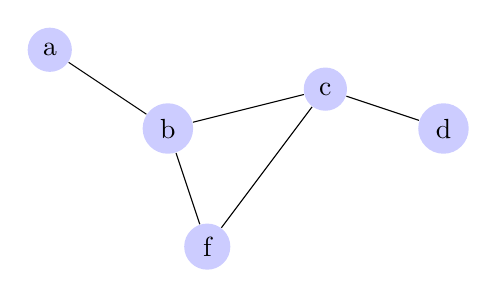
\begin{tikzpicture}
  [scale=.5,auto=left,every node/.style={circle,fill=blue!20}]
  \node (n6) at (1,10) {a};
  \node (n4) at (4,8)  {b};
  \node (n5) at (8,9)  {c};
  \node (n1) at (11,8) {d};
  \node (n3) at (5,5)  {f};

  \foreach \from/\to in {n6/n4,n4/n5,n5/n1,n5/n3,n3/n4}
    \draw (\from) -- (\to);

\end{tikzpicture}
    \caption{Ejemplo de subgráfica de G}
    \label{fig:SG}
\end{figure}
\end{center}
\begin{definition}
    Decimos que una subgráfica $H \subseteq G$ abarca $G$ (y $H$ es una subgráfica generadora de $G$) si cada vértice de $G$ está en $H$, i.e $V(H) = V(G)$\\
\end{definition}
\begin{center}
\begin{figure}[h]
    \centering
    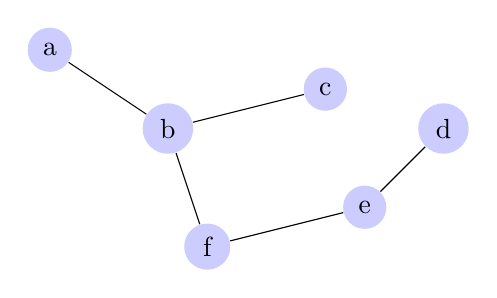
\begin{tikzpicture}
  [scale=.5,auto=left,every node/.style={circle,fill=blue!20}]
 \node (n6) at (1,10) {a};
  \node (n4) at (4,8)  {b};
  \node (n5) at (8,9)  {c};
  \node (n1) at (11,8) {d};
  \node (n2) at (9,6)  {e};
  \node (n3) at (5,5)  {f};

  \foreach \from/\to in {n6/n4,n4/n5,n3/n4,n3/n2,n2/n1}
    \draw (\from) -- (\to);

\end{tikzpicture}
    \caption{Ejemplo de una gráfica H que abarca G}
    \label{fig:GA}
\end{figure}
\end{center}
\newpage

\begin{definition} 
    Decimos que una subgráfica $H \subseteq G$, es una subgráfica inducida, si $E(H) = E(G) \cap E(V_H)$. En este caso $H$ es inducido por el conjunto $V(H)$ de vértices.
\end{definition}
\begin{center}
\begin{figure}[h]
    \centering
    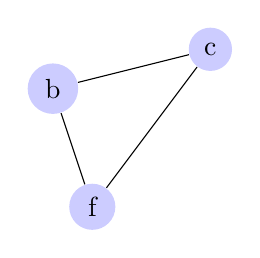
\begin{tikzpicture}
  [scale=.5,auto=left,every node/.style={circle,fill=blue!20}]
 
  \node (n4) at (4,8)  {b};
  \node (n5) at (8,9)  {c};
    \node (n3) at (5,5)  {f};

  \foreach \from/\to in {n4/n5,n3/n4,n5/n3}
    \draw (\from) -- (\to);

\end{tikzpicture}
    \caption{Ejemplo de una gráfica inducida}
    \label{fig:GI}
\end{figure}
\end{center}
 \subsection{Caminos y ciclos}
 Uno de los conceptos fundamentales que se introducirán y además se implmentarán en la creación de los algoritmos de la sección final es el concepto de caminos, este concepto se utilizará cómo herrramienta para el estudio y recorrido de la gráfica completa.

 \begin{definition}[Camino, ciclo y caminos cerrados]
    
     Sea $e_i = u_iu_{i+1} \in E(G)$ aristas de $G$ para $i \in \{1,...,k\}$. \\
     Un camino es una gráfica no vacía $W = (V,E)$ de la forma;
     \begin{center}
         $V = \{u_0,u_1,...,u_k,u_{k+1}\}$ \hspace{5pt} $E= \{e_0,e_1,...,e_k\}$
     \end{center}
     donde:
     $u_i$ es adyacente a $u_{i+1}$
     para todo $i \in \{1,...,k\}$.\\
     Además:
     \begin{enumerate}
         \item $W$ es \textbf{cerrado}, si $u_0 =u_{k+1}$.
         \item $W$ es un \textbf{camino}, si $u_i \neq u_j$, para todo $i \neq j$.
         \item W es un \textbf{ciclo}, si es cerrado y $u_i \neq u_j$ para $i \neq j$ excepto para $u_1 = u_{k+1}$
         
     \end{enumerate}
     
     Además, el número $l(W)$ es el tamaño o longitud del camino y está dado por $l(W)=|E(W)|$
 \end{definition}
 \subsection{Árboles}
 Una forma de reducir el número de vértices sin que la gráfica pierda gran parte de su información, es mediante el estudio de los árboles, veremos su definición y los conceptos más importantes relacionados con el estudio de estas estructuras.
  \begin{definition}[Gráfica conexa]
     Una gráfica $G=(V,G)$ es conexa si para cualquier par de vértices $u \hspace{5pt} y \hspace{5pt} v$ de G si existe un camino que inicia en $u$ y termina en $v$ \end{definition}
 \begin{definition}[Componente conexo]
     Sea $G=(V,E)$ una gráfica.
     Un \textbf{componente conexo} de $G$ es una subgráfica $H$ tal que:
     \begin{enumerate}
         \item $H$ es conexa.
         \item $H$ es maximal con respecto a la propiedad de ser conexa.Es decir, no existe una subgráfica conexa más grande  que contenga a $H$.
     \end{enumerate}
 \end{definition}
 \begin{definition}[Puente]
 Dada un gráfica $G$ conexa y una arista $e \in E_G$. Decimos que \textbf{e} es un puente de la gráfica $G$, si $G - e$ es disconexa.
 \end{definition}
 \noindent Si tomamos como ejemplo la gráfica de la figura \ref{fig:G} notamos que el vértice $e =ab$ es un puente de $G$.Pues la gráfica $G-e$ queda en dos componentes, la conformada por el vértice $\{a\}$ y la que contiene a los vértices $\{b,c,d,e,f\}$.
 
 \begin{proposition}
     Sea una gráfica $G$.
     Un vértice $e \in E(G)$ es un puente de $G$ si y sólo sí $e$ no está en ningún ciclo de $G$.
 \end{proposition}
 
 \begin{proof}
 Primero notemos que $e=uv$ es un puente sí y sólo sí $u$, $v$ pertenecen a diferentes componentes conexas de $G-e$, pues de lo contrario implicaría que existe un camino que conecta a $u$ con $v$ lo cual sería una contradicción ya que $G-e$ es disconexo.
 
     ($\Rightarrow$) Por contrapositiva, Supongamos que existe un ciclo de $G$ que contiene a $e$, entonces existe un camino tal que $C = \{u_0=u,v,...,u_{k+1}=u\}$.
     De aquí, notamos que en $G-e$ existe un camino $C' = \{v_0=v,...,v_{k+1} = u\}$,entonces existe un camino alterno que conecta a $u$ con $v$ lo cual implica que $G-e$ es conexa. Por tanto $e=uv$ no es puente.
     
     ($\Leftarrow$) Supongamos que $e=uv$ no es puente, por la observación hecha al inicio esto implica que $u$,$v$ pertenecen a la misma componente conexa de $G-e$.Entonces existe un camino que $C=\{v_0=v,...,v_{k+1} = u\}$ conecta a $v$ con $u$, de ahí notamos que $eC$ es un ciclo pues $eC = \{u,v_0=v,...,v_{k+1}=u\}$.
     \end{proof}
 

 \begin{definition}[Gráfica acíclica]
     Una gráfica es llamada acíclica si no contiene ciclos.
 \end{definition}
 \begin{definition}[Árbol]
  Un árbol es una gráfica acíclica y conexa.
 \end{definition}
 
 De la \textbf{Proposición 2.2} y la \textbf{Definición 22} se deriva el siguiente corolario.
 
 \begin{corollary}
     Una gráfica conexa es un árbol sí y sólo sí todas sus aristas son puentes.
 \end{corollary}
 \newpage
 



 \begin{teorema}
 Los siguientes enunciados son equivalentes:
  \begin{enumerate}
         \item $T$ es un arbol
         \item Cualesquiera dos vértices estan conectados en $T$ por un único camino.
         \item $T$ es aciclico y $\varepsilon_T = \nu_T - 1$
\end{enumerate}
     
 \end{teorema}
 
\begin{proof}
Sea \boldmath{$\nu_T$} = \textbf{n}, Si n=1 el teorema es trivial,así que supongamos para n $\geq$ 2.\\

    (1) $\Rightarrow$ (2) Supongamos que $T$ es un árbol. Sean $u$ y $v$ dos vértices de $T$ y por contradicción supongamos que existen dos caminos $P$ y $Q$ tales que conectan a \textbf{u} y \textbf{v}. Sin pérdida de generalidad supongamos que $l(P) > l(Q)$. Entonces existe al menos una arista \textbf{e} que está en $P$ pero no está en $Q$. Por \textbf{Corolario 2} sabemos que cada arista de $T$ es un puente. Y por lo visto anteriormente entonces \textbf{u} y \textbf{v} están en diferentes componentes conexas de $T-e$.Pero notamos que por el camino $Q$ siguen estando conectados. Lo cual es una contradicción ya que implicaria que \textbf{u} y \textbf{v} no estén en diferentes componentes conexas.\\

    (2) $\Rightarrow$ (3) Esta implicación la probaremos por inducción sobre \textbf{n}.
\\ Para $n=2$.
Sabemos que no existen componentes disconexas pues cualesquiera dos vértices están conectados por un camino, por lo cual $\varepsilon_T = 1 = 2-1= \nu_T -1$.
\\Supongamos que la afirmación se cumple para los valores menores a \textbf{n} y probemos para \textbf{n}.\\
Sea \textbf{P} el máximo camino en $T$ entre \textbf{u} y \textbf{v}, es decir que no existen aristas $e$ tales que $eP$  o $Pe$ sean caminos. De ahí que $d_T(v) = 1$.Si $uw \in E(T)$ entonces $w \in P$.
Ahora notamos que la subgráfica $T-v$ está conectada por un único camino $P'$ , además notamos que $l(P)$ es a lo más $n$ y cómo $l(P)>l(P')$ entonces $l(P') \leq n-1$ dado que la subgráfica $T-v$ esta conectada por un único camino (Pues $T$ lo está) y por hipotésis de inducción tenemos que:\\
\[\varepsilon_{T-v} = \nu_{T-v} - 1 = (n-1)-1 = n-2\]

Y de ahí que:
\[\varepsilon_T = \varepsilon_{T-v} + 1 = n-1\] \\
(3) $\Rightarrow$ (1) Supongamos (3). Basta con probar que $T$ es conexo.
Sean $T_i=(V_i,E_i)$ componentes conexos de $T$ para $i \in \{1,...k\}$. Sabemos que $T$ es acíclico,por lo tanto sus componentes conexos $T_i$ también los son por tanto $|E_i| = |V_i| - 1$.
Notemos que:
\begin{center}
    $\nu_T$ = $\sum_{i=1}^{k} |V_i|$
        ,
        $\varepsilon_T$ = $\sum_{i=1}^{k} |E_i|$
\end{center}
Entonces:

\begin{center}
    \[n-1 = \varepsilon_T = \sum_{i=1}^{k} (|V_i| - 1)= \sum_{i=1}^{k}|V_i| - k = n-k\] 
    \[\therefore k =1\]
\end{center}
Lo cual quiere decir que $T$ es un sólo componente conexo, por lo tanto $T$ es un árbol.





    
\end{proof}

\begin{definition}[Árbol generador]
    Dada una gráfica conexa $G$ una subgráfica $T$ de $G$ es un subárbol generado de $G$ si satisface que;

    \begin{enumerate}
        \item $T$ es una subgráfica generadora de $G$ y
        \item $T$ es un árbol.
    \end{enumerate}
\end{definition}
\begin{teorema}
    Cada gráfica conexa contiene un árbol generador.
\end{teorema}
\begin{proof}
    Sea $H\subset G$ la mínima gráfica generadora conexa de $G$, es decir $H-e$ es disconexa para todo $e \in E(H)$.
    Esta gráfica es obtenida de $G$ removiendo todas las aristas que no son puentes:
    \begin{enumerate}
        \item Hacemos $H_0 = G$.
        \item Para $i \geq 0$ sea $H_{i+1} = H_i - e_i$ donde $e$ no es un puente de $H_i$. Como $e_i$ no es un puente $H_{i+1}$ es una subgráfica generadora y conexa de $H_i$ y por lo tanto de $G$.
        \item De este forma hacemos $H = H_k$ cuando sólo quedan puentes en la subgráfica.
        Y por el \textbf{Coroloraio2} $H$ es un árbol.
    \end{enumerate}
\end{proof}

\begin{definition}[Árbol generador mínimo]
    
    Un árbol generador mínimo es un árbol generador tal que la suma de los pesos de sus aristas es la mínima posible, es decir.
\begin{center}
    $w(T) = \sum_{(u,v) \in T} min\{w(u,v)\}$
\end{center}
Donde $w(u,v)$ es el peso que hay entre el vértice $u$ y la arista $v$.
\end{definition}

Hablar de raices de un árbol dado que el mst se inicializa en una raíz

\begin{definition}[Característica de Euler]
    Dado un grafo plano $G$, la característica de Euler se define como:
    \begin{center}
        $\chi(G) = V-E+F$
    \end{center}
    Y esta propiedad es un \textbf{invariante topológico}.
    \newpage
    
\end{definition}
